\documentclass[a4paper,14pt]{extarticle}

\usepackage[utf8x]{inputenc}
\usepackage[T1]{fontenc}
\usepackage[russian]{babel}
\usepackage{hyperref}
\usepackage{indentfirst}
\usepackage{here}
\usepackage{array}
\usepackage{graphicx}
\usepackage{caption}
\usepackage{subcaption}
\usepackage{chngcntr}
\usepackage{amsmath}
\usepackage{amssymb}
\usepackage[left=2cm,right=2cm,top=2cm,bottom=2cm,bindingoffset=0cm]{geometry}
\usepackage{multicol}
\usepackage{multirow}
\usepackage{titlesec}
\usepackage{listings}
\usepackage{color}
\usepackage{enumitem}
\usepackage{cmap}
\usepackage{url}

\definecolor{green}{rgb}{0,0.6,0}
\definecolor{gray}{rgb}{0.5,0.5,0.5}
\definecolor{purple}{rgb}{0.58,0,0.82}

\lstdefinelanguage{none}{}

\lstset{
	language={Python},
	backgroundcolor=\color{white},
	commentstyle=\color{green},
	keywordstyle=\color{blue},
	numberstyle=\color{gray}\scriptsize\ttfamily,
	stringstyle=\color{purple},
	basicstyle=\lst@ifdisplaystyle\footnotesize\fi\ttfamily,
	breakatwhitespace=false,
	breaklines=true,
	captionpos=b,
	keepspaces=true,
	numbers=left,
	numbersep=5pt,
	showspaces=false,
	showstringspaces=false,
	showtabs=false,
	tabsize=4,
	frame=single,
	morekeywords={},
	deletekeywords={},
	extendedchars=false,
	columns=fullflexible,
	literate=%
		{~}{{\raise.25ex\hbox{$\mathtt{\sim}$}}}{1}%
		{-}{-}{1}
}

\titleformat*{\section}{\large\bfseries}
\titleformat*{\subsection}{\normalsize\bfseries}
\titleformat*{\subsubsection}{\normalsize\bfseries}
\titleformat*{\paragraph}{\normalsize\bfseries}
\titleformat*{\subparagraph}{\normalsize\bfseries}

\counterwithin{figure}{section}
\counterwithin{equation}{section}
\counterwithin{table}{section}
\newcommand{\sign}[1][5cm]{\makebox[#1]{\hrulefill}}
\newcommand{\equipollence}{\quad\Leftrightarrow\quad}
\newcommand{\no}[1]{\overline{#1}}
\newcommand{\code}[1]{\lstinline[language=none]|#1|}
\graphicspath{{../pics/}}
\captionsetup{justification=centering,margin=1cm}
\def\arraystretch{1.3}
\setlength\parindent{5ex}
\titlelabel{\thetitle.\quad}

\setitemize{topsep=0em, itemsep=0em}
\setenumerate{topsep=0em, itemsep=0em}


\begin{document}

\begin{titlepage}
\begin{center}
	Санкт-Петербургский Политехнический Университет Петра Великого\\[0.3cm]
	Институт компьютерных наук и технологий \\[0.3cm]
	Кафедра компьютерных систем и программных технологий\\[4cm]

	\textbf{ОТЧЕТ}\\
	\textbf{по лабораторной работе}\\[0.5cm]
	\textbf{<<Поиск векторов смещения>>}\\[0.1cm]
	Разработка графических приложений\\[3.0cm]
\end{center}

\begin{flushright}
	\begin{minipage}{0.5\textwidth}
		\textbf{Работу выполнил студент}\\[3mm]
		гр. 3540901/91502 \hfill \sign[1.1cm] \hfill Дьячков В.В.\\[5mm]
		\textbf{Работу принял преподаватель}\\[5mm]
		\sign[5cm] \hfill Абрамов Н.А. \\[5mm]
	\end{minipage}
\end{flushright}

\vfill

\begin{center}
	Санкт-Петербург\\[0.3cm]
	\the\year
\end{center}
\end{titlepage}

\addtocounter{page}{1}


\tableofcontents
\newpage

\section{Программа работы}

\begin{enumerate}
	\item Реализовать линейное растяжение гистограммы.
	\item Реализовать эквализацию гистограммы.
	\item Реализовать приведение гистограммы к заданной.
\end{enumerate}

\section{Выполнение работы}

\subsection{Линейное растяжение гистограммы}

Значение пикселя $p_{in}$ преобразуется в $p_{out}$ по формуле:
$$
p_{out} = (p_{in} - I_{low}) \cdot \frac{O_{high} - O_{low}}{I_{high} - I_{low}} + O_{low},
$$
где $I$ -- исходное изображение, а $O$ -- результирующее изображение.

При растяжении гистограммы используем $O_{high} = 255$ и $O_{low} = 0$, тогда
$$
p_{out} = (p_{in} - I_{low}) \cdot \frac{255}{I_{high} - I_{low}}
$$

\begin{figure}[H]
	\centering
	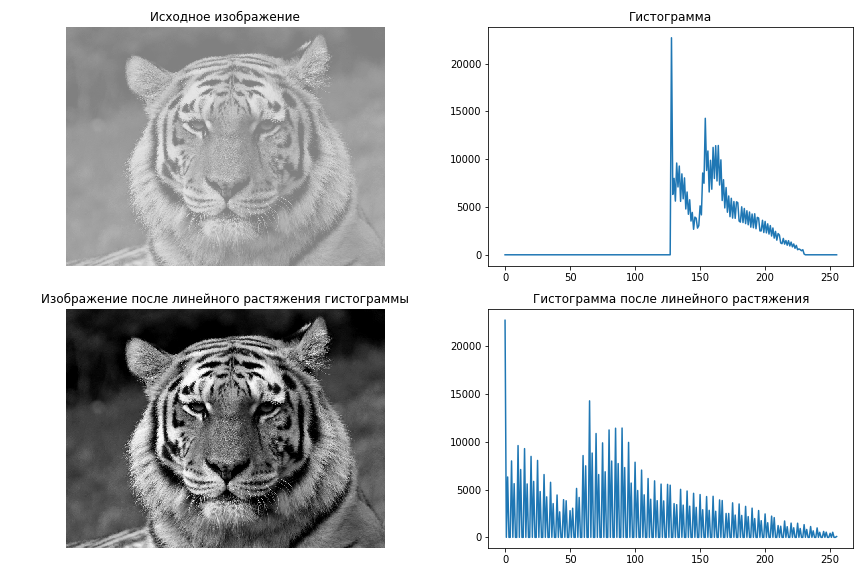
\includegraphics[width=\linewidth]{tiger_stretch}
	\caption{Линейное растяжение гистограммы (1)}
\end{figure}

\begin{figure}[H]
	\centering
	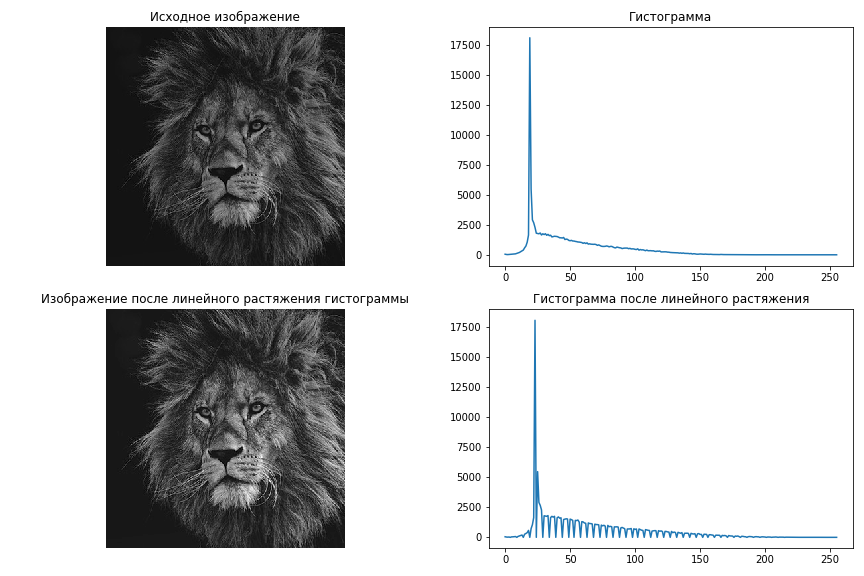
\includegraphics[width=\linewidth]{lion_stretch}
	\caption{Линейное растяжение гистограммы (2)}
\end{figure}

\begin{figure}[H]
	\centering
	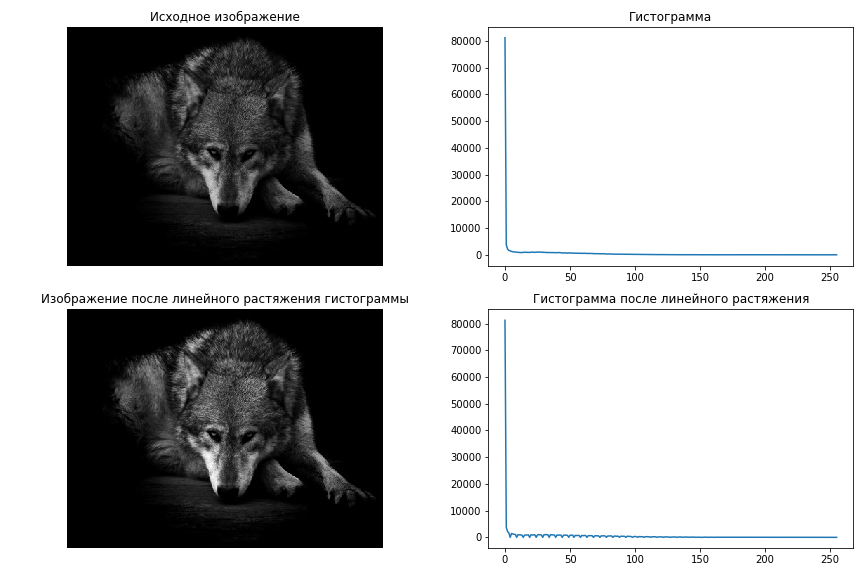
\includegraphics[width=\linewidth]{wolf_stretch}
	\caption{Линейное растяжение гистограммы (3)}
\end{figure}

\subsection{Устойчивое линейное растяжение гистограммы}

Попробуем применить устойчивое линейное растяжение гистограммы: будем отбрасывать $M\%$ (например, $5\%$) самых темных и самых светлых пикселей при подсчете минимума и максимума гистограммы исходного изображения. Это позволяет более устойчиво применить растягивание гистограммы, когда слишком светлых или слишком светлых пикселей небольшое количество.

\begin{figure}[H]
	\centering
	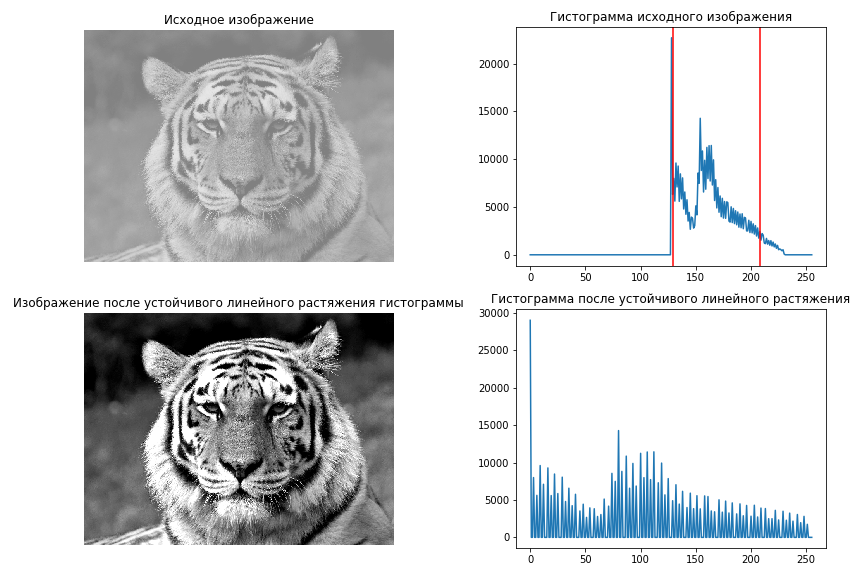
\includegraphics[width=\linewidth]{tiger_stretch_stable}
	\caption{Устойчивое линейное растяжение гистограммы (1)}
\end{figure}

\begin{figure}[H]
	\centering
	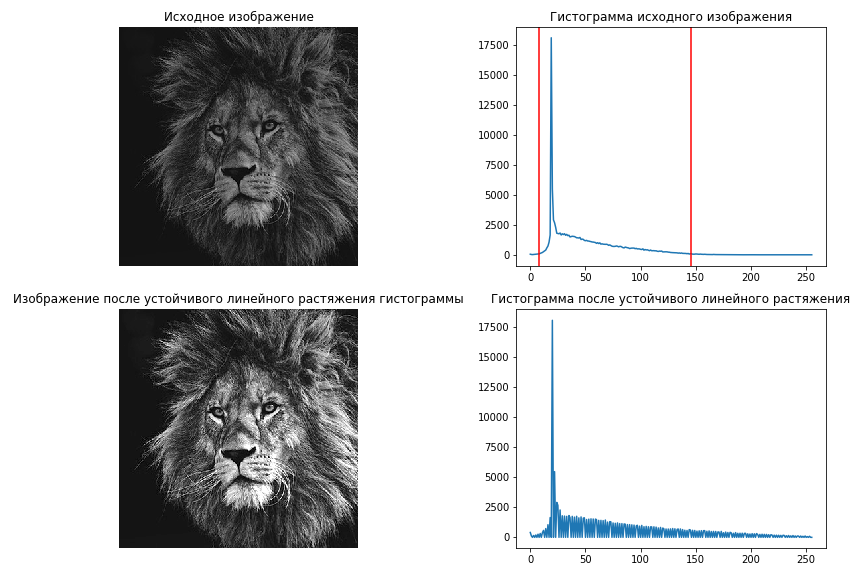
\includegraphics[width=\linewidth]{lion_stretch_stable}
	\caption{Устойчивое линейное растяжение гистограммы (2)}
\end{figure}

\begin{figure}[H]
	\centering
	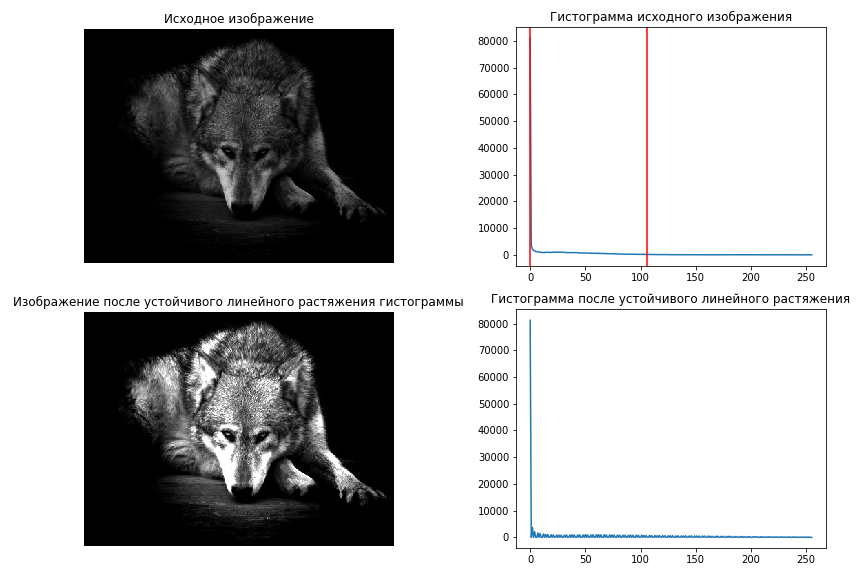
\includegraphics[width=\linewidth]{wolf_stretch_stable}
	\caption{Устойчивое линейное растяжения гистограммы (3)}
\end{figure}

\subsection{Эквализация гистограммы}

Применим другой метод повышения контрастности изображения -- эквализацию гистограммы. Определим функцию распределения $\mathit{cdf}(n) = h(0) + h(1) + ... + \mathit{cdf}(n)$. Другими словами, функция распределения является кумулятивной гистограммой. Наша задача сводится к тому, чтобы функция распределения имела вид, близкий к линейному, тогда пиксели изображения будут более равномерно использовать весь диапазон значений. Формула для преобразования пикселя входного изображения $p_{in}$:

$$
p_{out} = \mathit{round} \left( \frac{\mathit{cdf}(p_{in}) - \mathit{cdf}_{min}}{N} \cdot 255 \right),
$$

где $N$ -- общее число пикселей в изображении.

\begin{figure}[H]
	\centering
	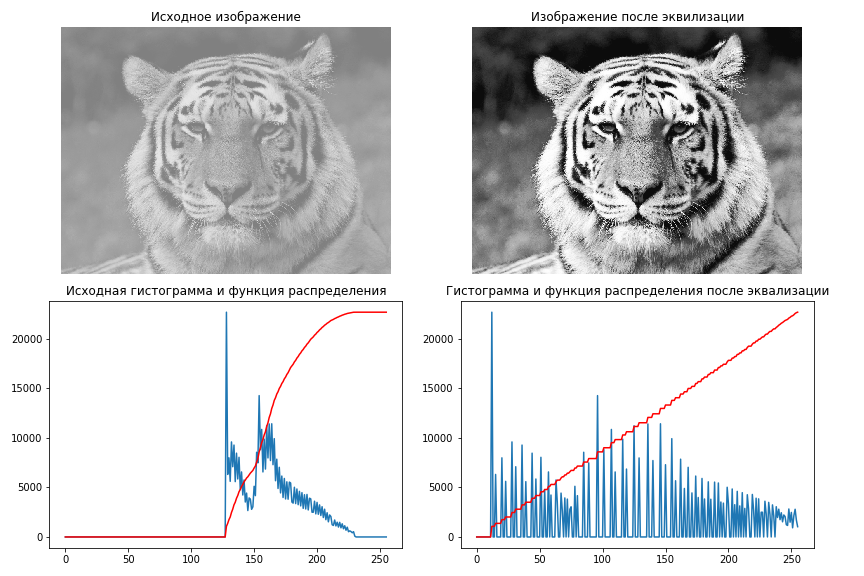
\includegraphics[width=\linewidth]{tiger_equalized}
	\caption{Эквализация гистограммы (1)}
\end{figure}

\begin{figure}[H]
	\centering
	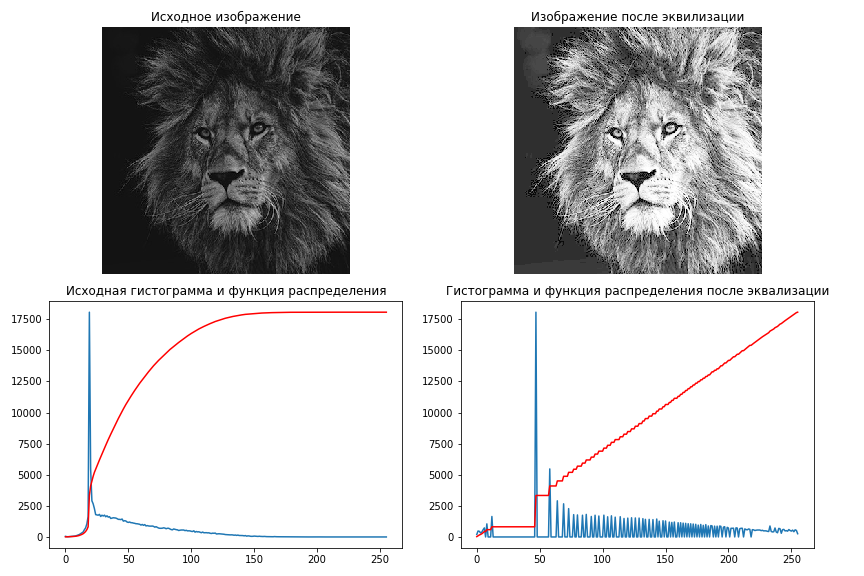
\includegraphics[width=\linewidth]{lion_equalized}
	\caption{Эквализация гистограммы (2)}
\end{figure}

\begin{figure}[H]
	\centering
	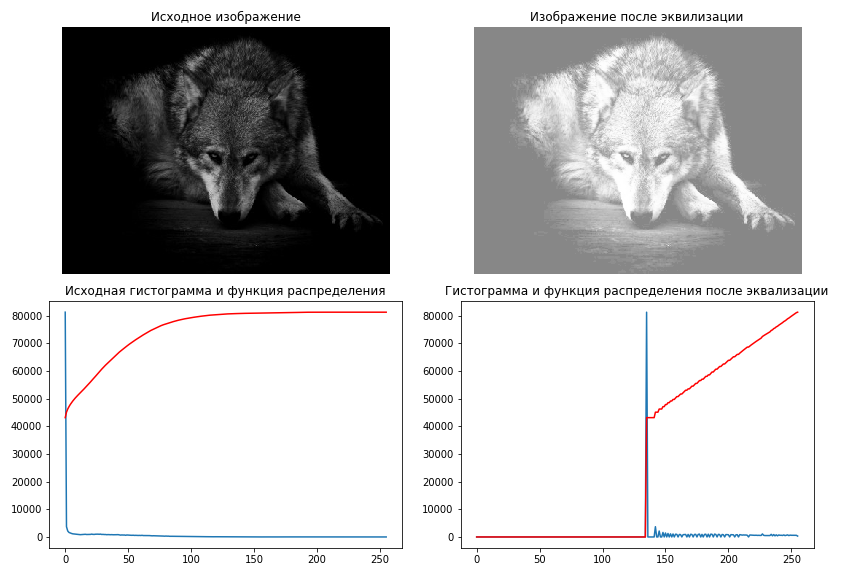
\includegraphics[width=\linewidth]{wolf_equalized}
	\caption{Эквализация гистограммы (3)}
\end{figure}

\subsection{Приведение гистограммы}

В том случае, если у нас есть референсное изображение, мы можем использовать его гистограмму для преобразования входного изображения. Для этого создадим отображение каждого значения входного изображения в выходное (всего 256 возможных входных и выходных значений), после чего отобразим значение каждого пиксель входного изображения в выходное. 

Рассчитаем гистограммы и функции распределений входного ($\mathit{cdf_1}$) и референсного ($\mathit{cdf_2}$) изображений, после чего найдем такие значения пикселей $p_1$ и $p_2$, что:
$$
\mathit{cdf_1}(p_1) = \mathit{cdf_2}(p_2),
$$
тогда значение пикселя $p_1$ отображается в значение $p_2$.

\begin{figure}[H]
	\centering
	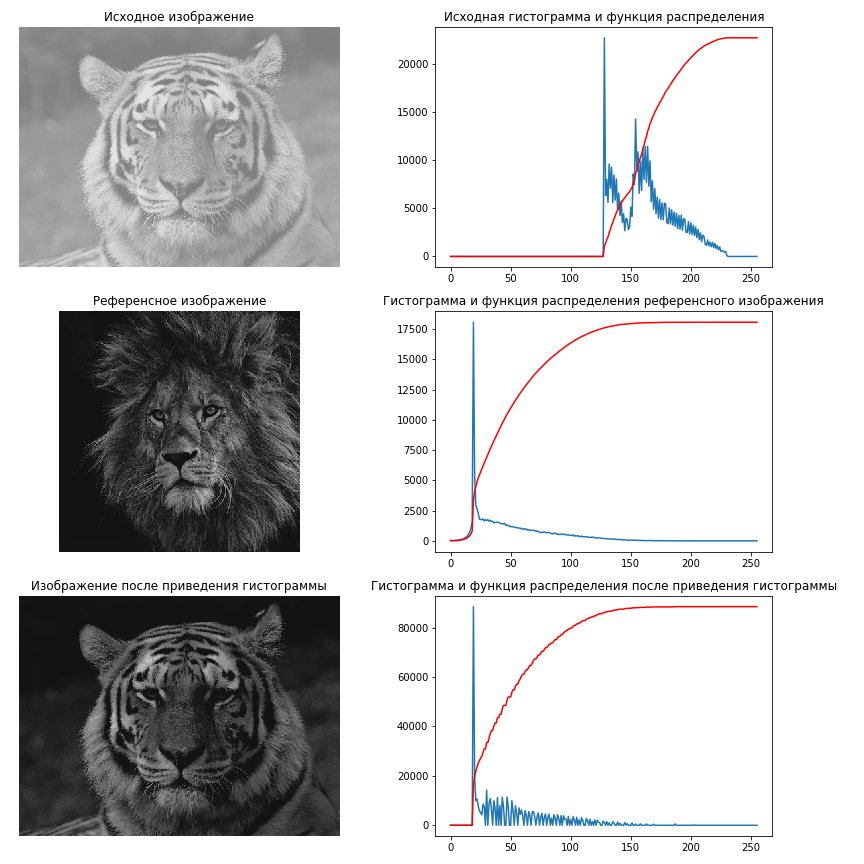
\includegraphics[width=\linewidth]{tiger_lion_matched}
	\caption{Приведение гистограммы (1)}
\end{figure}

\begin{figure}[H]
	\centering
	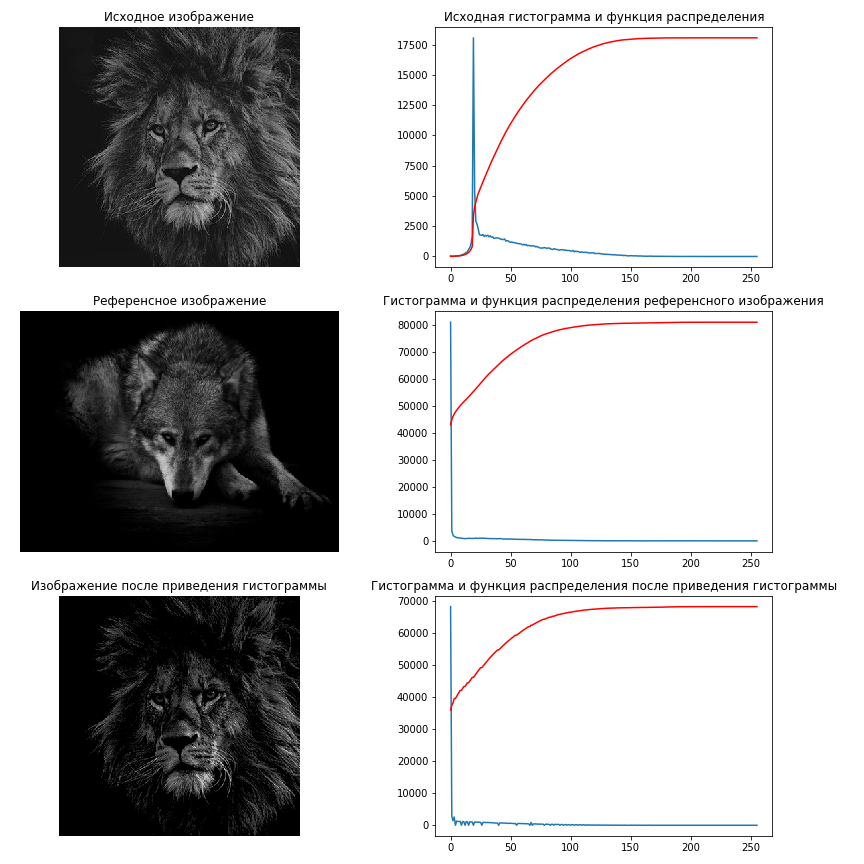
\includegraphics[width=\linewidth]{lion_wolf_matched}
	\caption{Приведение гистограммы (2)}
\end{figure}

\section{Выводы}

В данной работе были реализованы различные операции над гистограммой изображения:

\begin{itemize}
	\item линейное растяжение и устойчивое линейное растяжение гистограммы;
	\item эквализация гистограммы;
	\item приведение гистограммы изображения к заданному виду.
\end{itemize}

\end{document}